\chapter{Kerne}

\section{Kernmodelle}
Die Masse eines Kernes ist
\begin{equation*}
	m_\text{Kern} = Z\cdot m_\text{p} + N\cdot m_\text{n} - E_\text{B}
\end{equation*}
mit $Z$, der Kernladungszahl, $N$, der Neutronenzahl und $E_\text{B}$, der Bindungsenergie.

Es gibt verschiedene Modelle, diese Bindungsenergie zu beschreiben.

\subsection{Tröpfchenmodell}
Das Tröpfchenmodell beschreibt einen Atomkern wie einen Flüssigkeitstropfen.
Die darauf beruhende \textbf{Bethe-Weizsäcker-Massenformel} lautet
\begin{equation*}
	E_\text{B} = \underbrace{a_\text{V}A}_{E_\text{V}} - \underbrace{a_\text{S}A^\frac{2}{3}}_{E_\text{S}} - \underbrace{a_\text{C}\frac{Z(Z-1)}{A^\frac{1}{3}}}_{E_\text{C}} - \underbrace{a_\text{A}\frac{(A-2Z)^2}{A}}_{E_\text{C}} + \delta (A,Z).
\end{equation*}

\subsubsection{Der Volumenterm $E_\text{V}$}
Der Volumenterm $E_\text{V}$ ist proportional zum Volumen $V$ des Kerns, welcher proportional zu $A$ ist.
Es liegt dabei die starke Wechselwirkung zugrunde, die bekanntlich gleichermaßen auf Protonen und Neutronen wirkt, daher überrascht es nicht, dass kein $Z$ im Term vorkommt.
Die Zahl der möglichen Wechselwirkungspaare ist $\frac{A(A-1)}{2}$, also würde man naiv einen Term erwarten, der wie $A^2$ geht.
Allerdings hat die starke Wechselwirkung nur eine sehr begrenzte Reichweite, sodass nur nächste und übernächste Nachbarn wechselwirken können, daher geht der Term etwa linear in $A$.

\subsubsection{Der Oberflächenterm $E_\text{S}$}
Der Oberflächenterm $E_\text{S}$ basiert ebenfalls auf der starken Wechselwirkung.
Er ist eine Korrektur zum Volumenterm für Teilchen am Rand des Tropfens, der beachtet, dass Nukleonen an der Oberfläche des Tropfens weniger Wechselwirkungspartner zur Verfügung haben.
Wenn also das Volumen des Tropfens $\propto A$ ist, dann ist die Oberfläche $\propto A^\frac{2}{3}$, daher die Form.
Das Analogon zum Tropfen ist hier die Oberflächenspannung.

\subsubsection{Der Coulombterm $E_\text{C}$}
Dem Coulombterm $E_\text{C}$ liegt die elektrostatische Abstoßung zwischen den Protonen zugrunde.
Da die Abstoßung nur für mehr als ein Proton existieren kann, folgt die Form $Z(Z-1)$.
Wenn man annimmt, dass der Tropfen eine gleichmäßige Ladungsverteilung hat, so geht das elektrische Feld mit $\frac{1}{R}\propto\frac{1}{A^\frac{1}{3}}$.

\subsubsection{Der Asymmetrieterm $E_\text{A}$}
Beim Asymmetrieterm $E_\text{A}$ kommt das Pauli-Prinzip zum Tragen.
Sowohl Protonen, als auch Neutronen können unter Beachtung des Pauli-Prinzips innerhalb ihrer eigenen Pools Energieniveaus bis zu ihrer Fermienergie auffüllen.
Wenn nun von einer Sorte Nukleonen mehr Teilchen im Kern vorhanden sind, so hat dieser Pool eine höhere Fermienergie als der andere.
Wir könnten durch einen schwachen Zerfall nun die Energie senken, daher ist die Energie höher, als sie sein müsste.
Diese Überlegung bildet die Basis dieses Termes.

Im Fermigasmodell für Kerne folgt dieser Term sogar explizit aus der Rechnung.

\subsubsection{Der Paarungsterm $\delta$}
Dieser Term erfasst den Effekt der Spinkopplung und ist gegeben durch
\begin{equation*}
	\delta(A,Z) = \begin{cases}
									+\delta_0\quad\text{gg-Kerne} \\
									0 \quad\text{ug-Kerne} \\
									-\delta_0\quad\text{uu-Kerne} \\
								\end{cases}
\end{equation*}

\subsection{Das Fermigasmodell}
Im Fermigasmodell der Kerne betrachtet man die Neutronen und Protonen innerhalb des Kernes als (wechselwirkungsfreie), ideale Fermi-Gase bei $T=0$.
Gemäß den Lehren der statistischen Physik kann man somit die Fermienergie der Gase herleiten
\begin{equation*}
	\varepsilon_\text{n/p} = \left(\frac{9\pi}{4}\right)^\frac{2}{3} \frac{\hbar^2}{2m_\text{n/p}R_\text{s}^2}\left(\frac{\{N/Z\}}{A}\right)^\frac{2}{3}.
\end{equation*}

Der Asymmetrieterm im Tröpfchenmodell findet seine Begründung im Fermigas-Modell, wie bereits erläutert.
Man kann mit dem Fermigasmodell gut die Größenordnungen der Energien abschätzen, jedoch ist der Gültigkeitsbereich des Modells sehr beschränkt.
In einem nächsten Schritt könnte man die Wechselwirkung der Gase miteinbeziehen, was zu einer Korrektur führen würde.

\subsection{Schalenmodell}
Ein weiteres, sehr erfolgreiches Modell zur Beschreibung der Kerne ist das Schalenmodell.

\subsubsection{Magische Zahlen}
Experimentell beobachtet man, dass Kerne mit bestimmten Protonen- bzw. Neutronenzahlen besonders stabil sind.
Man nennt diese bestimmten Zahlen \textbf{magische Zahlen}.
Sie lauten
\begin{equation*}
	2, 8, 20, (28\text{, Neutronen}), 50, 82, 126 \dots
\end{equation*}
Außerordentlich stabil sind dabei \textbf{doppelt-magische} Kerne.
Diese Tatsache suggeriert Schalenabschlüsse, wie im Atommodell, allerdings gibt es hier den Unterschied, dass es kein dominierendes Zentralpotenzial gibt.

\subsubsection{Das Modell}
Man betrachtet die Zustände eines Nukleons in einem von den anderen Nukleonen erzeugten Feld.
Jeder Zustand ist dabei nach dem Pauli-Prinzip besetzt.

Setzt man ein radialsymmetrisches, im Inneren konstantes und scharfrandiges Potenzial an, so faktorisiert die Schrödingergleichung in einen Radial- und Winkelanteil.
Am besten scheint experimentell dabei ein Fermi-ähnliches Potenzial zu passen, das \textbf{Woods-Saxon-Potenzial}
\begin{equation*}
	V(r) = -\frac{V_0}{1+e^\frac{r-R}{a}}.
\end{equation*}
Leider ist dieses Potenzial analytisch nicht lösbar, weshalb man ein ähnlich verlaufendes, modifiziertes, harmonisches Potenzial verwendet.

Jedenfalls erhält man als Lösungen der Schrödingergleichung diskrete Energieniveaus, die je nach Quantenzahlen bestimmte Anzahlen an Teilchen aufnehmen können
\begin{equation}\label{eq:eniveaus}
	E_{n,l} = \hbar\omega\left(2(n-1) + l + \frac{3}{2}\right).
\end{equation}
Die ersten 3 magischen Zahlen können so durch die Auffüllung der Energieniveaus erklärt werden, jedoch ab der vierten nicht mehr.
Daher kann ein reines Zentralpotenzial nicht die Lösung sein.

Hier muss nun die Spin-Bahn-Kopplung der Nukleonen miteinbeziehen
\begin{equation*}
	\tilde{V}(r) = V_0(r) + V_{ls}(r)\frac{\mvec{l}\cdot\mvec{s}}{\hbar^2}.
\end{equation*}
\textbf{Nach \autoref{eq:eniveaus} ist $l$ allerdings nicht wie beim Atommodell nach oben durch $n$ beschränkt, sondern kann beliebige Werte annehmen!}
Daher ist die Spin-Bahn-Kopplung im Kern insbesondere für große $l$ sehr groß!

Mit diesem Modell können nun alle magischen Zahlen erklärt werden, da Niveaus mit größerem Gesamtdrehimpuls hier energetisch günstiger sind.
Atome wollen also den Gesamtdrehimpuls minimieren, während Kerne ihn maximieren wollen.

\section{Instabile Kerne}
Instabile Kerne können über verschiedene Zerfälle in stabile Kerne zerfallen.

\subsection{$\upgamma$-Strahlung}
Angeregte Kerne verlieren überschüssige Energie durch monoenergetische Photonenemission.
Da die elektromagnetische Wechselwirkung paritätserhaltend und drehimpulserhaltend ist, müssen sogenannte \textbf{Auswahlregeln} beachtet werden
\begin{equation*}
	|J_f-J_i|\leq l\leq J_f+ J_i\quad (0\rightarrow 0\ \text{aber verboten!}).
\end{equation*}

\subsection{$\upbeta$-Zerfall}
\begin{figure}
	\centering
	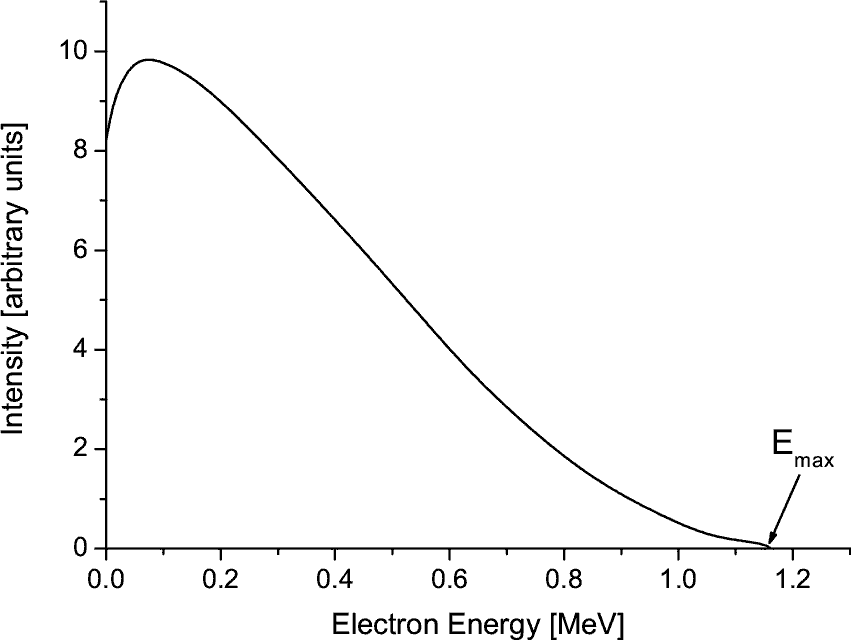
\includegraphics[width=.5\textwidth]{./img/betaspec.jpg}
	\caption{Elektronspektrum des Betazerflls von Bi-210}
	\label{fig:betaspec}
\end{figure}
Kerne können über die schwache Wechselwirkung einen $\upbeta$-Zerfall ausführen und zerfallen in ein Isotop der benachbarten Elemente.
Da der $\upbeta$-Zerfall ein 2-Körperzerfall ist, ist das Elektronspektrum kontinuierlich, da sich der Impuls auf das Neutrino und das Elektron verteilen kann, wie man in \autoref{fig:betaspec} sehen kann.

\subsection{$\upalpha$-Zerfall}
Kerne können sich auch über die Emission eines He-4 Kernes umwandeln.
Das dabei emittierte Alphateilchen ist monoenergetisch und die Energie hängt von der Energiebilanz (Bindungsenergien) und der Masse des Kernes ab.

\subsection{Anwendung: CNO-Zyklus}
\begin{figure}
	\centering
	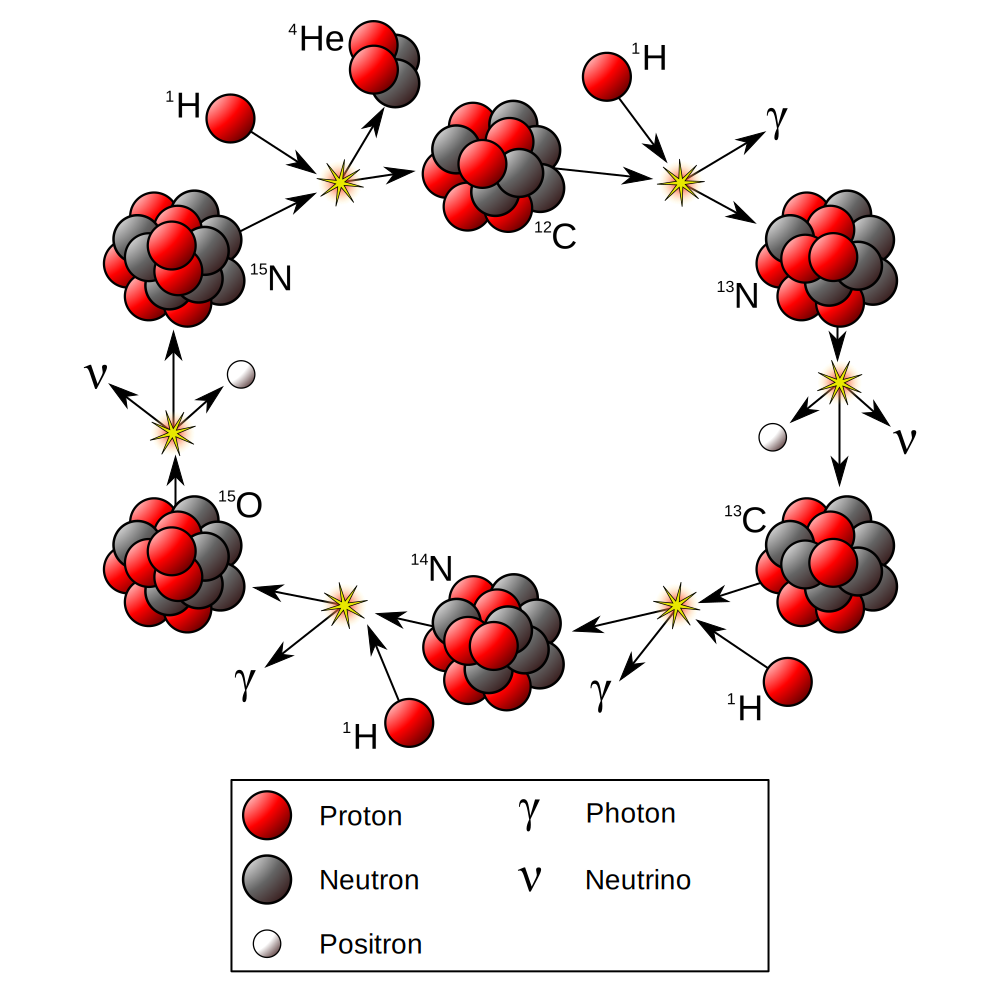
\includegraphics[width=.5\textwidth]{./img/cno.pdf}
	\caption{Der CNO-Zyklus}
	\label{fig:cno}
\end{figure}
Der CNO-Zyklus ist eine der acht Fusionsreaktionen des so genannten Wasserstoffbrennens, durch die Sterne Wasserstoff in Helium (und dann in schwerere Elemente) umwandeln.
Er ist in \autoref{fig:cno} abgebildet.

\subsection{Anwendung: Big-Bang-Nucleosynthesis}
Direkt nach dem Urknall war das Universum sehr dicht und sehr heiß.
Das Verhältnis von Protonen und Neutronen (aus dem Quark-Gluon-Plasma am Anfang) war im thermischen Gleichgewicht etwa 1:1, da die dominanten Übergänge
\begin{align*}
	n + \pos &\rightleftharpoons \bar{\nu_e} + p \\
	n + \nu_e &\rightleftharpoons p + \el
\end{align*}
aufgrund der hohen Temperatur und Dichte schnell abgelaufen sind.

Während der Abkühlung ($t<\SI{1}{\second}$) jedoch tendierte das Gleichgewicht immer mehr zu den Protonen, da diese eine etwas kleinere Masse als Neutronen haben.
Das Universum kühlte sich immer weiter ab und das Verhältnis \nicefrac{n}{p} sank immer weiter, bis die Temperatur und Dichte zu niedrig waren und damit die Reaktionen zu langsam abliefen.
Zu diesem Zeitpunkt war das Verhältnis bei etwa \nicefrac{1}{6}.
Da freie Neutronen instabil mit einer Halbwertszeit von $\SI{880}{\second}$ sind, zerfielen noch ein paar Neutronen bevor sie sich zu Kernen binden konnten
\begin{equation*}
	n \longrightarrow p + \el + \bar{\nu_e}.
\end{equation*}
Damit war das Verhältnis schlussendlich bei etwa \nicefrac{1}{7} angekommen.

Da He-4 die größte Bindungsenergie unter den leichten Elementen hat, verbanden sich die Neutronen überwiegend zu He-4-Kernen.
